%ju 28-Mai-22 FM_U08_Leistung_Loesung.tex
\section{Leistung Übung 8}\label{leistung-uebung-8}

\textbf{Aufgabe 1}

\begin{figure}[!ht]% hier: !ht
\centering
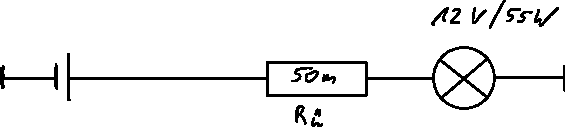
\includegraphics[width=0.6\textwidth]{images/Skizze/26_FM_Nr8_Leistung_A1.pdf}
\caption{FM Nr8 Leistung A1}
%\label{fig:}%% anpassen
\end{figure}

\lstset{language=Python}% C, TeX, Bash, Python 
\begin{lstlisting}[
	%caption={}, label={code:}%% anpassen
][language=Python]
# geg:
U_ges = 14,8 V
R_u = 0,05 Ohm = 50 mOhm
P_La = 55 W
U = 12 V
# ges: P_La_tat
# Formel:
P_La = U x I -> P_La = U^2/R_La -> R_La = U^2/P_La
R_ges = R_u + R_La
I_tat = U_ges/R_ges
P_La_tat = U_k x I_tat -> P_La_tat = R_La x I_tat^2
# Lösung:
R_La = 2,6182 Ohm
R_ges = 2,6682 Ohm
I_tat = 5,5468 A
P_La_tat = 80,555 W
\end{lstlisting}

\textbf{Aufgabe 2}

\lstset{language=Python}% C, TeX, Bash, Python 
\begin{lstlisting}[
	%caption={}, label={code:}%% anpassen
][language=Python]
# geg:
R = 50 Ohm
P = 500 W
# ges: I
# Formel:
P = U x I -> P = R x I^2 -> I = sqrt(P/R)
# Lösung:
I = 3,1623 A
\end{lstlisting}

\newpage

\textbf{Aufgabe 3}

\begin{figure}[!ht]% hier: !ht
\centering
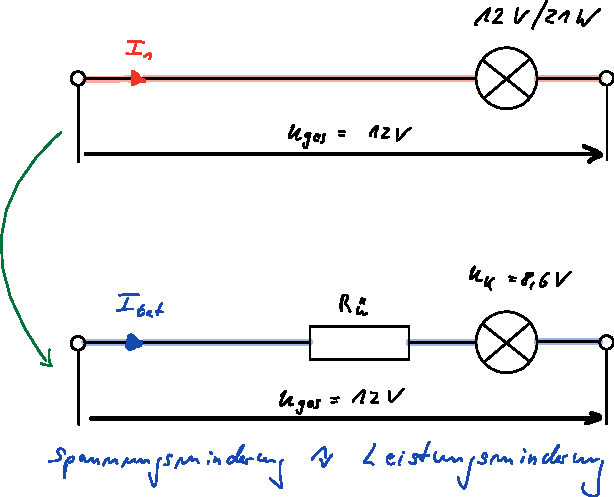
\includegraphics[width=0.6\textwidth]{images/Skizze/26_FM_Nr8_Leistung_A3.pdf}
\caption{FM Nr8 Leistung A3}
%\label{fig:}%% anpassen
\end{figure}

\lstset{language=Python}% C, TeX, Bash, Python 
\begin{lstlisting}[
	%caption={}, label={code:}%% anpassen
][language=Python]
# geg:
U_ges = 12 V
P_La = 21 W
U_k = 8,6 V
# ges: R_u, P_R_u, P_La_tat
# Formel:
P_La = U x I -> P_La = U^2/R_La -> R_La = U_ges^2/P_La
I_tat = U_k/R_La
R_u = U_R_u/I_tat -> R_u = (U_ges - U_k)/I_tat
P_R_u = U_R_u x I_tat ->
P_R_u = R_u x I_tat^2
P_La_tat = U_k x I_tat
# Lösung:
R_La = 6,8571 Ohm
I_tat = 1,2542 A
R_u = 2,711 Ohm
P_R_u = 4,2642 W
P_La_tat = 10,7858 W
\end{lstlisting}

\newpage

\textbf{Aufgabe 4}

\textbf{Durch welche technische Größe kommt es bei einer 24 V Glühlampe
zur gleichen Leistung wie bei einer 12 V Glühlampe, obwohl doch die
äußerlichen Baugrößen identisch sind?}

\begin{figure}[!ht]% hier: !ht
\centering
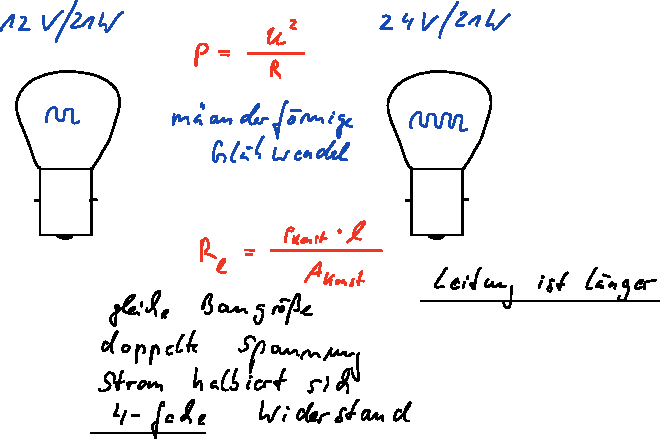
\includegraphics[width=0.6\textwidth]{images/Skizze/26_FM_Nr8_Leistung_A4.pdf}
\caption{FM Nr8 Leistung A4}
%\label{fig:}%% anpassen
\end{figure}

\lstset{language=Python}% C, TeX, Bash, Python 
\begin{lstlisting}[
	%caption={}, label={code:}%% anpassen
][language=Python]
# geg:
P = 21 W
U_1 = 12 V
U_2 = 24 V
# Formel:
P = U x I -> P = U^2/R ->
R_1 = U_1^2/P
R_2 = U_2^2/P
Faktor = R_2/R_1
# Lösung:
12V/21W R_1 = 6,8571 Ohm
24V/21W R_2 = 27,4286 Ohm
Faktor = 4 - fache Widerstand
\end{lstlisting}

Bei einer 24 V Lampe ist der Widerstand viermal größer als bei einer 12
V Glühlampe. Dieser Widerstand liegt hierbei an einer doppelten Spannung
gegenüber der 12 V Spannung. Durch die doppelte Spannung und dem
vierfachen Widerstand stellt sich ein Strom ein, der die Hälfte
gegenüber einer Spannung von 12 V hat.

Somit ergibt sich die gleiche Leistung bei 24 V. Um diesen Widerstand zu
erhalten, vierfache Leiterlänge, ist die Glühwendel mäanderförmig
gefertigt in dem Glaskolben verlegt.

\textbf{Aufgabe 5}

\textbf{Wenn man ein 12 V Bordnetz mit einem 24 V Bordnetz vergleicht,
stellt man in der Dimensionierung der verlegten elektrischen Leitung
kein Unterschied fest. Ist die oben genannte Aussage zutreffend, oder
gibt es ihrer Meinung nach doch ein Unterschied in der Dimensionierung
der Leitungen?}

Die Spannung ist höher, demzufolge kann die Stromstärke kleiner sein,
ergo können auch die Leitungen in ihrer Fläche kleiner sein, da die
Belastung nicht so groß ist.

Da der Stromfluss durch die Leitungen geringer ist, tritt an diesen
Leitungen auch nicht ein so großer Spannungsverlust auf. Dadurch tritt
an dem zu schaltenden Verbraucher auch nicht eine so hohe
Spannungsminderung der Klemmenspannung auf.
